\chapter{经验研究}\label{sec:study}

本章将主要介绍为了解当前漏洞数据库现状,考察其中漏洞补丁的质量和特征所开展的经验研究工作,包括:经验研究的设计、数据准备以及经验研究的结果分析。


\section{研究设计}
\subsection{研究问题}
为了了解已有漏洞数据库中开源软件漏洞补丁的质量和特征,本文所开展的针对当前\tocheck{高质量}漏洞数据库的经验研究包含以下研究问题:

\begin{itemize}[leftmargin=*]
    \item \textbf{RQ1 覆盖率分析:}当前\tocheck{高质量}漏洞数据库中,漏洞补丁信息的覆盖度如何?即:有多少漏洞包含补丁信息?(Sec. \ref{sec:coverage})
    \item \textbf{RQ2 一致性分析:}不用漏洞库间,漏洞补丁信息的一致性如何?即:有多少漏洞在漏洞数据库中具有相同的补丁信息?(Sec. \ref{sec:consistency})
    \item \textbf{RQ3 补丁类型分析:}开源漏洞补丁的类型有哪些? (Sec. \ref{sec:type})
    \item \textbf{RQ4 补丁映射分析:}开源漏洞与其补丁在数量上的映射关系是怎样的? (Sec. \ref{sec:cardinality})
    \item \textbf{RQ5 补丁准确性分析:}当前\tocheck{高质量}漏洞数据库中,漏洞的补丁信息准确度如何? (Sec. \ref{sec:accuracy})
\end{itemize}
    
其中,RQ1可用来评估漏洞数据库中开源软件漏洞的补丁缺失程度,RQ2用来评估不同漏洞数据库中漏洞补丁的不一致程度,RQ3和RQ4用来表征常见的补丁类型以及开源漏洞及其补丁之间的映射关系,RQ5可用来评估不同漏洞数据库中漏洞补丁信息的准确性。总的来说,RQ1、RQ2和RQ5的结果旨在从不同的角度评估补丁质量,并挖掘出对自动化补丁\tocheck{识别}方法的需求;RQ3和RQ4旨在从不同角度捕捉开源软件漏洞补丁的特征,并为自动化补丁\tocheck{识别}方法的设计提供\tocheck{启发}。

\subsection{评估标准}\label{sec:metric}
本章经验研究使用了信息检索中常用的评估标准---Precision(精确率)、Recall(召回率)和F1-Score(F1值)。

对于一个搜索或分类问题来说,样本分为“Positive(正)”和“Negative(负)”两个类别。那么,模型搜索或分类的结果就会有四种情况:
\begin{itemize}
    \item True Positive(真阳性),表示:将正样本预测为正样本,即数据库提供的或工具返回的正确补丁信息。
    \item True Negative(真阴性),表示:将负样本预测为负样本,即数据库未提供的或工具未返回的错误补丁信息。
    \item False Positive(假阳性),表示:将负样本预测为正样本,即数据库提供的或工具返回的错误补丁信息。
    \item False Negative(假阴性),表示:将正样本预测为负样本,即数据库未提供的或工具未返回的正确补丁信息。
\end{itemize}

\textbf{Precision(精确率),}用于衡量数据库提供的补丁中正确补丁的比率,或是工具返回结果中正确补丁的比率,计算公式如下:
\begin{equation}\label{eq:precision}
    Precision=\frac{True\ Positive}{True\ Positive + False\ Positive} 
\end{equation}

\textbf{Recall(召回率),}用于衡量正确补丁在数据库中被提供的比率,或是正确补丁被工具返回的比率,计算公式如下:
\begin{equation}\label{eq:recall}
    Recall=\frac{True\ Positive}{True\ Positive + False\ Negative} 
\end{equation}

\textbf{F1-Score(F1值),}用以中和表示Precision及Recall的结果;因为Precision仅仅反映精确率,Recall仅仅反映召回率,无法反映总体评估结果,F1-Score计算公式如下:
\begin{equation}\label{eq:f1}
    F1-Score=2*\frac{Precision*Recall}{Precision + Recall} 
\end{equation}

\section{数据准备}\label{sec:preparation}
\subsection{漏洞数据库选择}
为挑选高质量的、具有代表性的漏洞数据库作为研究对象,本文前期调研了来自安全领域的社区、工业界和学术界的漏洞数据库。在该章节的经验研究工作中,本文首先排除了来自安全社区的数据库(例如,CVE List和NVD)。因为这两个数据库不提供结构化的补丁信息,而补丁链接多是隐藏在参考链接中;此外,CVE List和NVD数据库中不仅仅包含开源软件漏洞,还包括闭源软件、系统及硬件相关的漏洞。本文还排除了来自学术界的数据集\cite{ponta2019manually,fan2020ac,jimenez2018enabling,gkortzis2018vulinoss,namrud2019androvul,li2017large,liu2020large,antal2020exploring},这是因为这些数据集中的漏洞通常限定于特定的一两种程序语言(例如:Python、Java),而非面向所有开源软件,缺乏多样性不具有代表性;此外,由于长期缺乏维护,这些漏洞数据集缺失较新的漏洞数据。


对于工业界的数据库,本文首先关注到BlackDuck\cite{blackduck}、WhiteSource\cite{whitesource}、Veracode\cite{veracode}和Snyk\cite{snyk}四家安全公司提供软件成分分析(Software Composition Analysis)服务,这种服务通过识别并分析当前软件系统中使用的开源成本(即:第三方库),报告所使用的开源成分中的漏洞。因此,这四家公司需要先构建尽可能完整且包含详细漏洞信息的漏洞库作为服务基础,本文便首先将这四家公司的漏洞数据库作为研究对象。截至2021年4月5日,收集的信息为:

\begin{itemize}[leftmargin=*]
\item\textbf{Black Duck,}该公司的报告显示:该公司的安全公告中共包含157,000多个漏洞,涵盖90多种编程语言,其中,数千个漏洞尚未被NVD收录。该公司的漏洞数据库由特定的专家团队进行维护,以确保漏洞数据的完整性和准确性,然而,该公司的漏洞数据信息并未对外公开。
\item\textbf{Sonatype\footnote{https://ossindex.sonatype.org},} 该公司声称:\textit{“OSS Index是一个免费的开源组件目录,其中的扫描工具可帮助开发人员识别漏洞、了解风险并确保其软件安全。”}\footnote{英文原文为:"OSS Index is a free catalogue of open source components and scanning tools to help developers identify vulnerabilities, understand risk, and keep their software safe."} Sonatype的OSS Index支持20多个生态系统(如:Maven、npm、Go、PyPI等)。该公司公开的漏洞信息包括:漏洞描述、受漏洞影响的组件和版本、CVSS向量和参考链接等信息。
\item\textbf{WhiteSource\tocheck{链接},}该公司从NVD及其他安全公告平台和问题追踪系统(issue tracking system)中共收集的漏洞超过175,000个,涵盖200多种编程语言。
\item\textbf{Veracode\tocheck{链接},}该公司的漏洞数据库涵盖10多种编程语言相关的18,000多个漏洞,公开的漏洞信息包括:受漏洞影响的组件和版本范围、库修复说明、参考资料等。
\item\textbf{Snyk\footnote{https://snyk.io/vuln},}该公司声称:漏洞数据库\footnote{https://snyk.io/product/vulnerability-database/}是由经验丰富的安全研究团队持续维护,通过关注安全公告、Jira issue报告,Github commits等方式自动识别安全漏洞相关的报告。该公司的数据库涵盖超过10个编程语言生态系统,如:Maven、npm、Go、Composer等。该数据库提供漏洞的详细信息,包括:受漏洞影响的组件、版本范围、修复方法、参考链接等。
% \item \textbf{Gitlab Security} GitLab 咨询数据库是 Gitlab 依赖扫描器\footnote{https://docs.gitlab.com/ee/user/application\_security/dependency\_scanning/index.html} 的基础。目前涵盖了 6000 多个 CVE 条目和 8 个生态系统(即 Nuget、Conan、Maven 等)。提供了详细信息,例如描述、受影响的组件和版本、解决方案和参考。
\end{itemize}

进一步调研后发现,这四家公司中某些公司并未公开漏洞数据库,或是公开的漏洞信息中不包含用于修复漏洞的补丁信息,这将无法达成研究目标。最终,本文选定Veracode和Snyk的漏洞数据库作为研究对象,下文中简称为:$DB_A$和$DB_B$。


\subsection{广度数据集构建}
为了评估漏洞数据库中补丁的缺失程度以及不同数据库间补丁的不一致性(即:RQ1和RQ2),本文基于$DB_A$和$DB_B$构建了一个开源软件漏洞的广度数据集用以实验分析。截至2020年4月7日,分别从$DB_A$和$DB_B$中分别获取了\tocheck{8,630}和\tocheck{5,858}个CVE漏洞。

\subsection{深度数据集构建}
为了表征漏洞补丁的类型、映射关系以及尽可能准确地评估补丁信息的准确性(即:RQ3、RQ4和RQ5),本文还基于$DB_A$和$DB_B$的数据,构建了一个开源软件漏洞的深度数据集。该数据集的漏洞数量少于广度数据集,但每个漏洞都包含由人工确认的补丁信息。%为了确保漏洞补丁信息完整性和准确性,其中所有漏洞的补丁信息都是由人工识别。

在该深度数据集的构建过程中,为了确保数据集能够涵盖足够多的漏洞用以实验评估,但又不至于在人工识别补丁的阶段产生难以完成的工作量,本文仅将在$DB_A$和$DB_B$都含有补丁信息的漏洞列入该深度数据集,最终,该深度数据集共包含\tocheck{1,417}个CVE漏洞。



然后,对于该深度数据集中的每个CVE漏洞,首先分别由两位研究人员通过分析$DB_A$和$DB_B$数据库报告的补丁、查看NVD中的漏洞描述和参考链接信息以及搜索GitHub代码仓库的提交历史和其他网络资源等方式,独立得找到其补丁信息;之后,对比由两位研究人员独立查找得到得补丁信息,对于补丁结果不一致的漏洞,两位研究人员再一起分析讨论直到达成共识。这两位研究人员分别是本文作者和与本文作者同课题组的学生。由于公开的信息有限,\tocheck{1,417}个CVE漏洞中的\tocheck{122}个CVE漏洞无法找到补丁信息,比如:漏洞CVE-2016-3942在NVD中没有漏洞报告,但$DB_A$和$DB_B$将 jsrender@f984e1\cite{jsrender}标识为其补丁,两位研究人员无法确认该补丁信息的准确性。最终,该深度数据集共包含了\tocheck{1,295}个CVE漏洞。

\begin{figure*}[h]
    \centering
    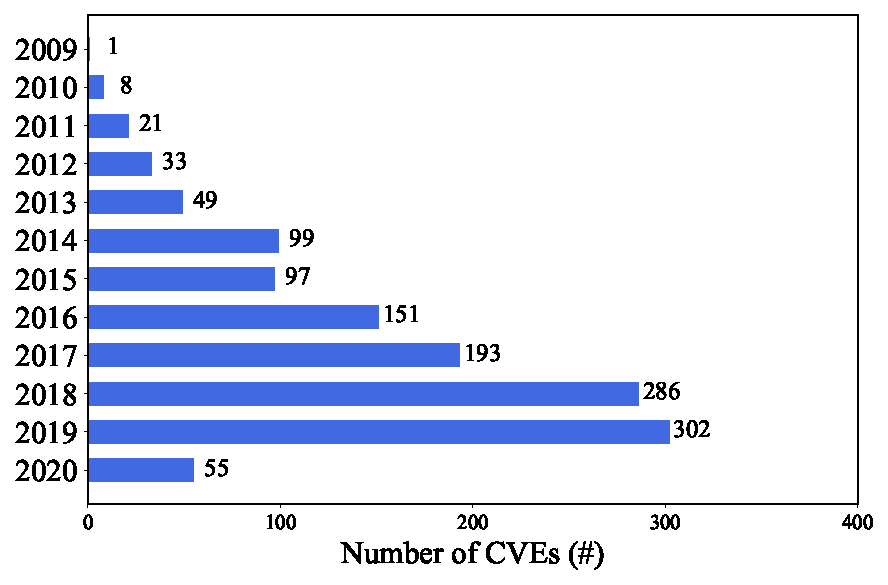
\includegraphics[scale=0.66]{res/rq0-year.pdf}
    %\vspace{-5pt}
    \caption{数据集中漏洞年份统计}\label{fig:rq0-year}
\end{figure*}


% \begin{figure*}[h]
%     \centering
%     \begin{subfigure}[b]{0.45\textwidth}
%     \centering
%     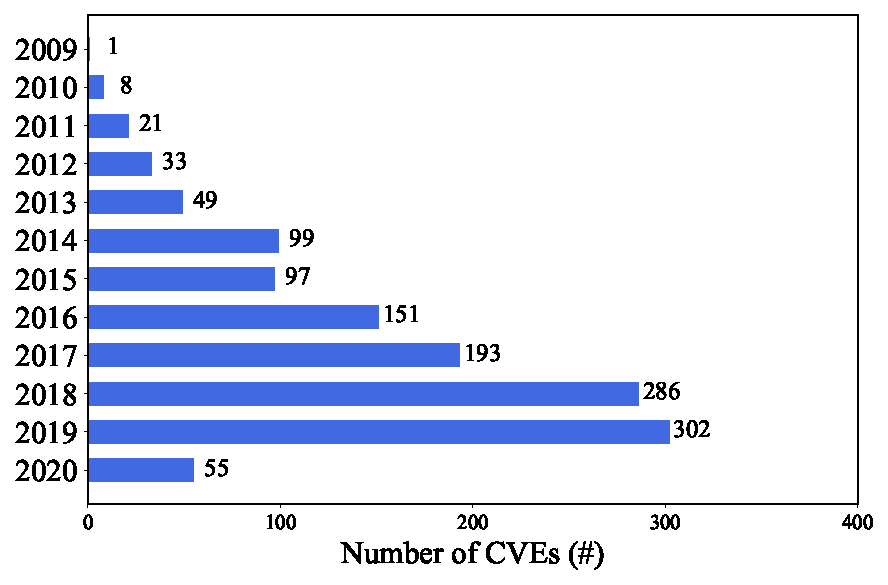
\includegraphics[scale=0.46]{res/rq0-year.pdf}
%     %\vspace{-5pt}
%     \caption{漏洞年份分布统计}\label{fig:rq0-year}
%     \end{subfigure}
%     \begin{subfigure}[b]{0.45\textwidth}
%     \centering
%     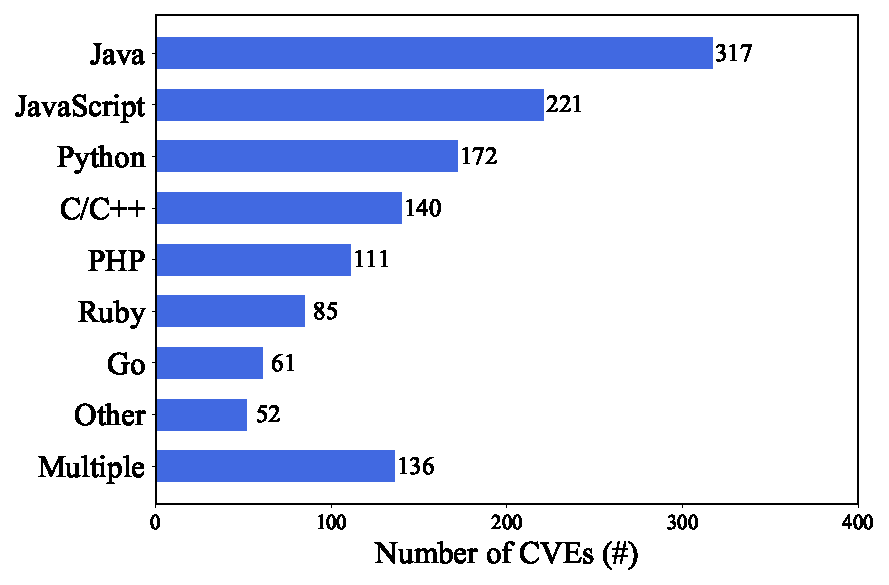
\includegraphics[scale=0.46]{res/rq0-language.pdf}
%     %\vspace{-5pt}
%     \caption{程序语言分布统计}\label{fig:rq0-language}
%     \end{subfigure}
%     %\vspace{-20pt}
%     \caption{数据集中漏洞年份及程序语言分布统计}\label{fig:dataset}
% \end{figure*}



\begin{figure*}[h]
    \centering
    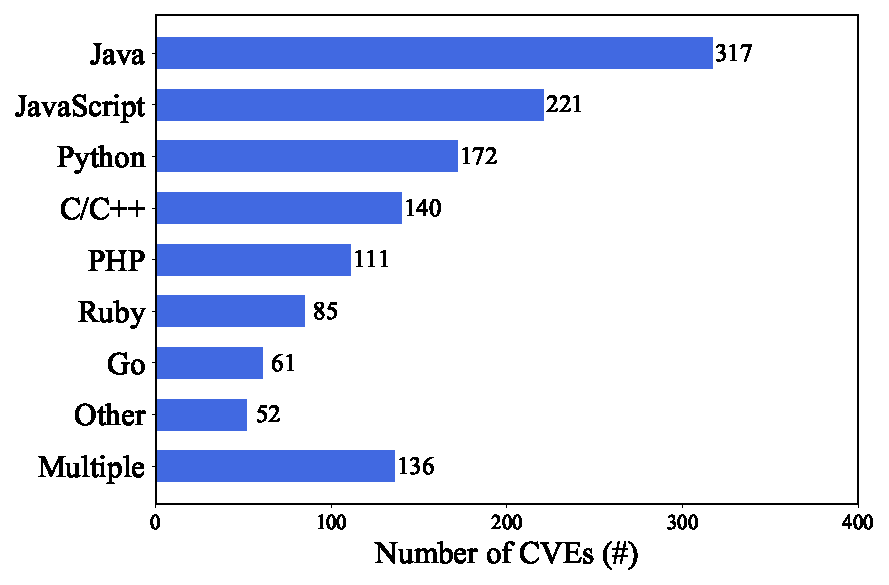
\includegraphics[scale=0.68]{res/rq0-language.pdf}
    \caption{数据集中漏洞程序语言分布统计}\label{fig:rq0-language}
\end{figure*}


本文还进一步分析了该深度数据集中\tocheck{1,295}个CVE开源软件漏洞的年份和程序语言分布情况,以评估该数据集是否具有代表性。如图\ref{fig:rq0-year}所示,CVE的数量逐年增加,这与Snyk的报告\cite{Snyk-report}一致。此外,本文通过分析补丁中更改的源文件类型来确定CVE的编程语言。如图\ref{fig:rq0-language}所示,深度数据集中的CVE漏洞涵盖了七种较为常用的程序语言,具有较好的语言多样性。因此,可以认为该深度数据集对于开源软件漏洞数据库具有较好的代表性。


\section{RQ1:覆盖率分析}\label{sec:coverage}
\begin{figure}[h]
    \centering
    \begin{subfigure}[b]{0.45\textwidth}
    \centering
    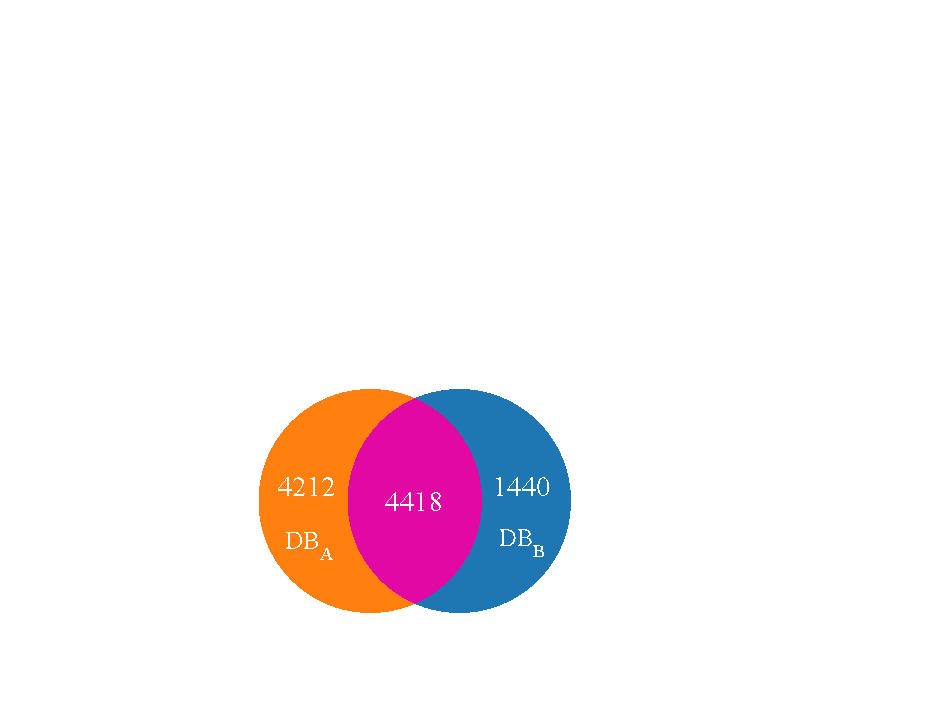
\includegraphics[scale=0.98]{res/rq1-CVE-IDs-VS.pdf}
    %\vspace{-5pt}
    \caption{开源软件漏洞}\label{fig:rq1-cves}
    \end{subfigure}
    \begin{subfigure}[b]{0.45\textwidth}
    \centering
    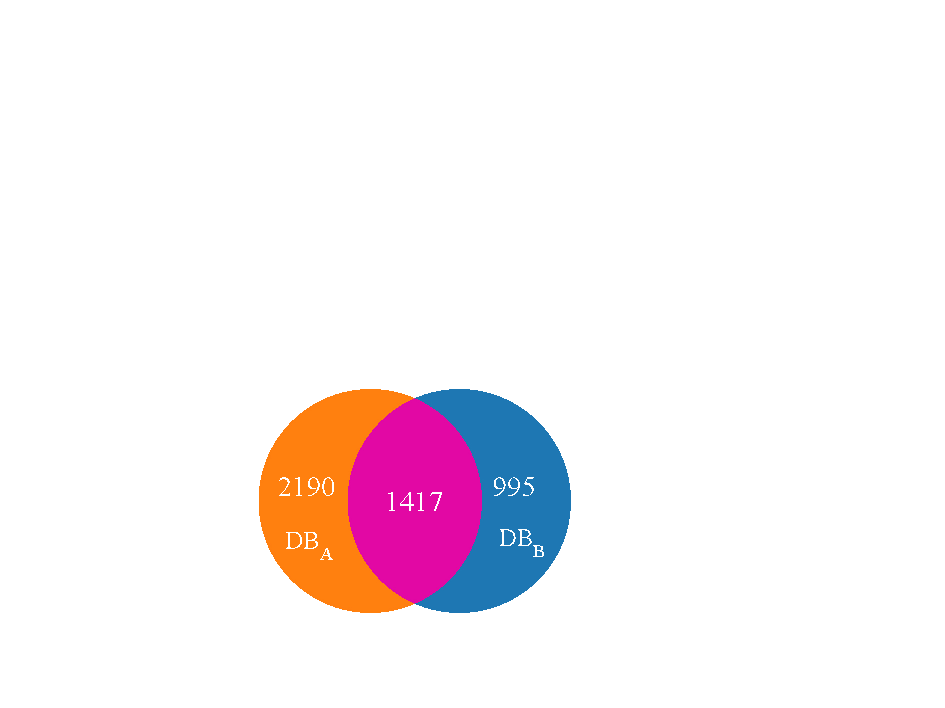
\includegraphics[scale=0.98]{res/rq1-CVE-IDs-Patches-VS.pdf}
    %\vspace{-5pt}
    \caption{含补丁信息的开源软件漏洞}\label{fig:rq1-cves-with-patches}
    \end{subfigure}
    %\vspace{-10pt}
    \caption{$DB_A$与$DB_B$间数据交集}\label{fig:intersection}
\end{figure}


如图\ref{fig:rq1-cves}所示,$DB_A$和$DB_B$数据库中共有的CVE漏洞为\tocheck{4,418}个,同时$DB_A$和$DB_B$分别包含\tocheck{4,212}和\tocheck{1,440}个特有的CVE漏洞;如图\ref{fig:rq1-cves-with-patches}所示,$DB_A$中\tocheck{3,607(41.8\%)}的CVE漏洞含有补丁信息,$DB_B$中\tocheck{2,412(41.2\%)}的CVE漏洞含有补丁信息;$DB_A$和$DB_B$数据库共有\tocheck{10,070}个开源软件CVE漏洞,而其中仅有\tocheck{4,602(45.7\%)}的漏洞提供了补丁信息。

% \begin{figure}[h]
%     \centering
%     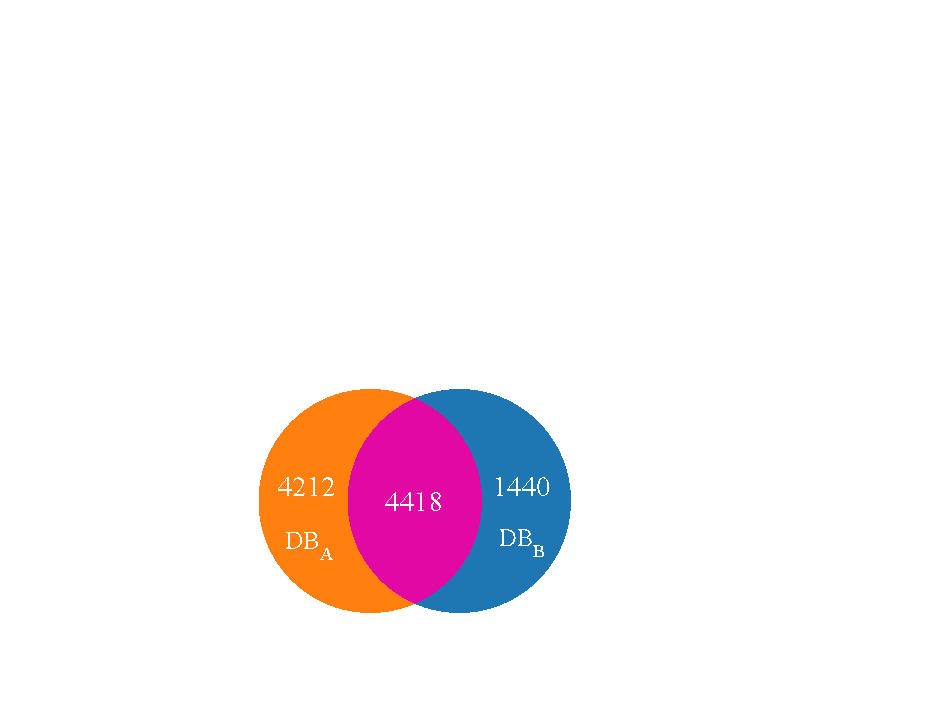
\includegraphics[scale=0.98]{res/rq1-CVE-IDs-VS.pdf}
%     \caption{开源软件漏洞数据}\label{fig:rq1-cves}
% \end{figure}

% \begin{figure}[h]
%     \centering
%     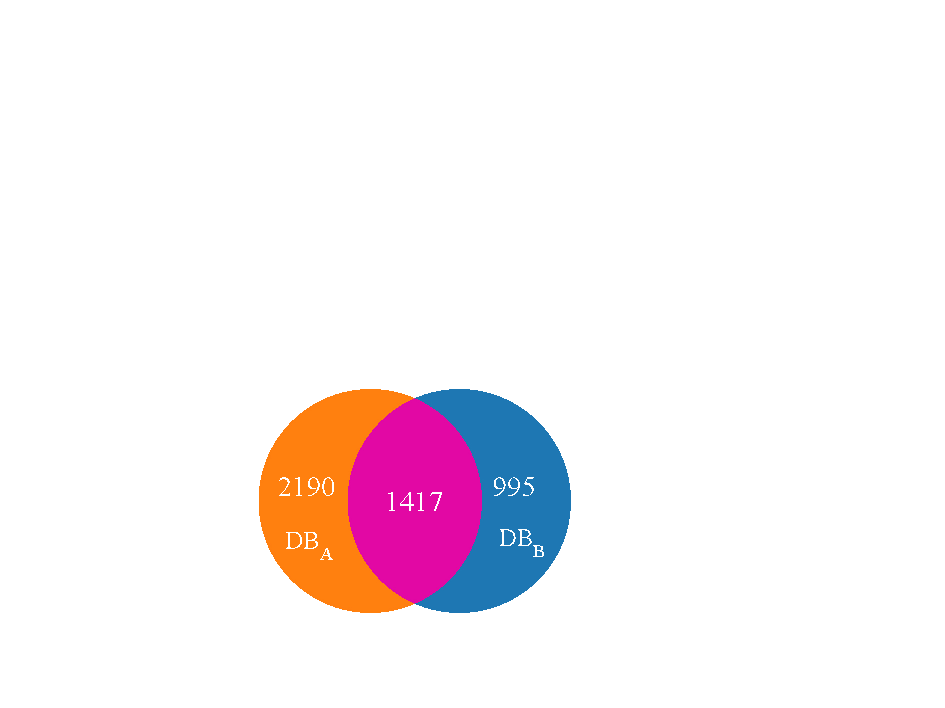
\includegraphics[scale=0.98]{res/rq1-CVE-IDs-Patches-VS.pdf}
%     \caption{补丁信息的开源软件漏洞数据}\label{fig:rq1-cves-with-patches}
% \end{figure}

由此可见,数据库$DB_A$和$DB_B$中开源软件漏洞的补丁覆盖率都较低,分别为41.8\%和41.2\%,漏洞补丁缺失的情况较为普遍。%而且可以看出,不同的漏洞数据库对\congyingEdit{OSS}漏洞的覆盖范围不同。
同时,这也体现出自动化补丁查找方法的必要性,可用于填补数据库中缺失的补丁信息。


\section{RQ2:一致性分析}\label{sec:consistency}

\begin{table}[h]
    \centering
    \footnotesize
    \caption{补丁一致性结果}\label{table:consistency}
    %\vspace{-10pt}
    \begin{tabular}{|*{1}{C{5.0em}}|*{1}{C{5.0em}}*{1}{C{5.5em}}*{1}{C{5.5em}}|*{1}{C{5.0em}}*{1}{C{5.0em}}*{1}{C{5.0em}}|}
    \noalign{\hrule height 1pt}
    \multirow{2}{*}{补丁一致} & \multicolumn{3}{c|}{存在性不一致} & \multicolumn{3}{c|}{内容不一致} \\\cline{2-4}\cline{5-7}
     & 总数 & 无漏洞信息 & 无补丁信息 & 总数 & 包含关系 & 非包含关系 \\\noalign{\hrule height 1pt}
    % \multirow{2}{*}{Cons.} & \multicolumn{3}{c|}{Existence Inconsistency} & \multicolumn{3}{c|}{Content Inconsistency} \\\cline{2-4}\cline{5-7}
    % & Total & No CVE & No Patch & Total & Inclusion & Difference \\\noalign{\hrule height 1pt}
    907 (19.7\%) & 3,185 (69.2\%) & 1,392 (30.2\%) & 1,793 (39.0\%) & 510 (11.1\%) & 176 (3.8\%) & 334 (7.3\%)\\
    % $DB_{A}$ vs. $DB_{C}$ & 3,659 & 73 (2.0\%) & 3,540 (96.7\%) & 2,523 (69.0\%) & 1,017 (27.8\%) & 46 (1.3\%) & 15 (0.4\%) & 31 (0.8\%) \\
    % $DB_{B}$ vs. $DB_{C}$ & 2,490 & 75 (3.0\%) & 2,397 (96.3\%) & 1,687 (67.8\%) & 710 (28.5\%) & 18 (0.7\%) & 7 (0.3\%) & 11 (0.4\%)\\
    \noalign{\hrule height 1pt}
    \end{tabular}
\end{table}

为了分析两个数据库之间的补丁信息一致性情况,本节主要关注带有补丁的CVE漏洞,即:图\ref{fig:rq1-cves-with-patches}中的CVE漏洞。考虑到漏洞补丁的个数可能不唯一(即:可能为一组补丁集),所以仅当两个数据库针对同一漏洞提供的补丁集完全相同时,才判定为补丁信息一致。本节将补丁信息不一致分为存在性不一致和内容不一致两种情况。前者是指某一个数据库为该CVE漏洞提供了补丁信息,而另一个数据库却不存在该CVE信息,或是存在该CVE却不存在相关补丁信息;后者是指两个数据库都存在该CVE的补丁信息,但它们的补丁集并不完全一致,分为包含关系或非包含关系的不一致。这两种情况分别反映了出数据库$DB_A$和$DB_B$中开源软件漏洞及其补丁信息的不完整性,以及漏洞补丁信息可能是不准确的


表\ref{table:consistency}中展示了补丁一致性分析的结果。其中,第一列为在$DB_A$和$DB_B$中具有一致补丁集的CVE数量(907,19.7\%),第二至四列为补丁存在性不一致的CVE数量(3,185,69.2\%),最后三列为都存在补丁信息但补丁集内容不一致的CVE数量(510,11.1\%)。可以发现:\tocheck{4,602}个CVE中,(1)只有\tocheck{907(19.7\%)}的漏洞在$DB_A$和$DB_B$中有一致的补丁信息;(2)超过三分之二(即:\tocheck{3,185(69.2\%)})的CVE漏洞在数据库$DB_A$和$DB_B$中存在补丁信息不一致的情况,其中\tocheck{1,392(30.2\%)}的CVE漏洞不在$DB_{A}$或$DB_{B}$中,\tocheck{1,793(39.0\%)}的CVE漏洞都存在于$DB_{A}$和$DB_{B}$中但在某一数据库中无补丁信息;(3)\tocheck{510(11.1\%)}的CVE漏洞补丁信息都存在于$DB_{A}$和$DB_{B}$中补丁集内容不一致,其中,\tocheck{176(3.8\%)}CVE的来自于某一个数据库的补丁集包含来自另一个数据库的补丁集,\tocheck{334(7.3\%)}CVE的来自$DB_{A}$和$DB_{B}$的补丁集即不同也不包含。

这些结果表明,$DB_A$和$DB_B$间存在较多的补丁信息不一致情况,进而表明数据库中补丁信息的准确性也需要进一步评估。


\section{RQ3:补丁类型分析}\label{sec:type}

在\tocheck{\ref{sec:preparation}小节}中,基于人工收集的深度数据集共包含\tocheck{1,295}个CVE漏洞及\tocheck{3,043}个补丁,本小节将基于该数据集分析漏洞的补丁类型。分析结果表明,\tocheck{3,043}个补丁中,\tocheck{2,852(93.7\%)}的补丁都是为GitHub commit形式,这可能是因为GitHub在开源软件中被广泛使用;另外\tocheck{136(4.5\%)}的补丁为SVN commit形式,仅有\tocheck{55(1.8\%)}的补丁为来自其他Git平台的commit形式。

此外,从CVE的角度来看,\tocheck{1,295}个CVE中\tocheck{1,202(92.8\%)}的CVE有GitHub commit类型的补丁,\tocheck{4(0.3\%)}的CVE有SVN commit类型的补丁。由于很多项目是从SVN切换为Git管理,\tocheck{48(3.7\%)}的CVE既有GitHub commit又有SVN commit类型的补丁。只有\tocheck{30(2.3\%)}的CVE的补丁都为来自其他Git平台的commit形式。以上分析结果表明,开源软件漏洞的补丁类型主要为GitHub commit,少部分为SVN commit,而极小部分为其他Git平台的commit。

\section{RQ4:补丁映射分析}\label{sec:cardinality}
\begin{figure}[h]
\centering
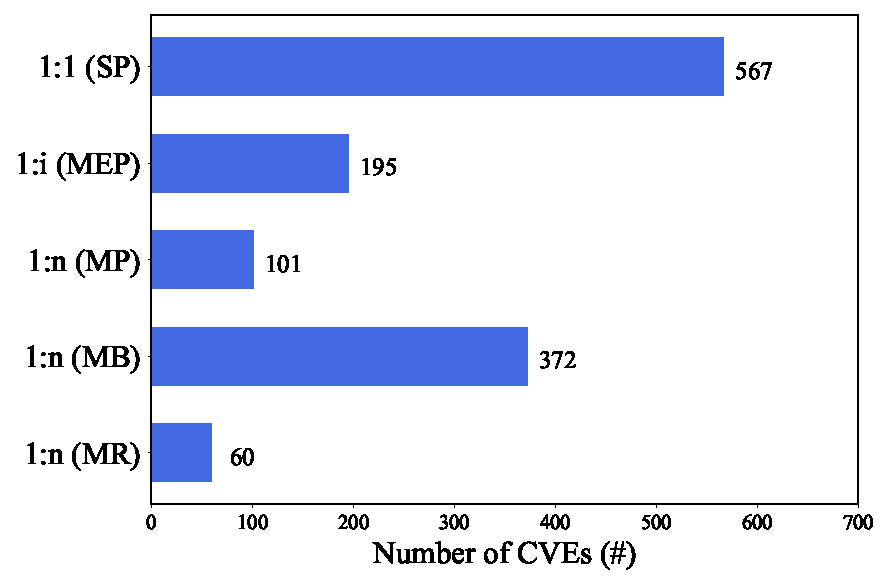
\includegraphics[scale=0.68]{res/rq4-cardinality.pdf}
\vspace{-10pt}
\caption{Mapping Cardinalities between CVEs and Patches}\label{fig:rq4-cardinality}
\end{figure}

基于深度数据集中\tocheck{1,295}个CVE漏洞及其补丁数据,本节将分析开源漏洞及其补丁间在数量上的映射关系。本文将CVE与其补丁之间的映射关系分为三种类型:一对一、\tocheck{一对一组}及一对多。

\textbf{一对一,}是指一个CVE漏洞与其补丁在数量上为一对一的关系,即:一个CVE漏洞只需一个补丁即可修复,后文中简记为:\textit{SP}(Single Patch)。如图\ref{fig:rq4-cardinality}所示,深度数据集中\tocheck{567(43.8\%)}的CVE与其补丁具有一对一的映射关系(\textit{SP})

\textbf{\tocheck{一对一组},}是指一个CVE漏洞有多个补丁信息,CVE漏洞与其补丁(commit)在数量上非一对一关系,然而,这些commit又都是等效的,任何一个补丁都足以修复该漏洞,后文中简记为:\textit{MEP}(Multiple Equivalent Patch)。等效补丁,是指代码变更完全一样的两个commit,其主要有两种类型:(1)Requested Commit VS. Merged Commit,通过GitHub中的Pull Request功能修补的CVE漏洞,请求提交(requested commit)和合并提交(merged commits)是该漏洞的等效补丁集。例如,python-jose@89b463\cite{python-jose-1}是拉取请求提交(requested commit),python-jose@73007d\cite{python-jose-2}是用于修复CVE-2016-7036的合并提交(merged commits),这两个commit是等效的。(2)SVN Commit VS. Github Commit,一些开源软件的仓库是后期由SVN迁移到GitHub的,因此,同一软件的SVN和GitHub的代码仓库中分别有用于修补该CVE的commit,且这两处的commit中代码变更是完全一样且完全等效的。例如,james-hupa代码仓库从SVN迁移到了GitHub,SVN commit james-hupa@1373762\cite{james-hupa-1}与GitHub commit james-hupa@aff28a\cite{james-hupa-2}是等效的。
如图\ref{fig:rq4-cardinality}所示,深度数据集中\tocheck{195(15.1\%)}的CVE与其补丁为一对一组映射关系(\textit{MEP})

\textbf{一对多,}是指一个CVE漏洞与其补丁在数量上为一对多的关系,即:个CVE漏洞需多个非等效的补丁来修复。如图\ref{fig:rq4-cardinality}所示,深度数据集中\tocheck{533(41.2\%)}的CVE与其补丁为一对多的映射关系,其可以再分为三种类型: 

\begin{itemize}[leftmargin=*]
\item 一个CVE是通过一个分支中的多个独立commit来修复的。这是因为该CVE较难修复需多次提交(commit),或是后期发现初始的补丁不足以修复漏洞便追加了补丁。后文中将此简记为:\textbf{\textit{Multiple Patch,MP}},占比\tocheck{7.8\%(101)}。例如,CVE-2017-17837由三个独立的提交deltaspike@4e2502\cite{deltaspike-1}、deltaspike@72e607\cite{deltaspike-2}和deltaspike@d95abe\cite{deltaspike-3} 修复。
\item 一个CVE由多个分支中的多个补丁集修复。这是因为该漏洞影响了开源软件的多个版本,而每个版本又都在独立的分支上维护。后文中将此简记为:\textbf{\textit{Multiple Branches,MB}},占比\tocheck{28.7\%(372)}。例如,CVE-2019-19118影响了django框架的2.1.x、2.2.x、3.0.x和3.2.x版本,提交django@103ebe\cite{django-1}、django@36f580\cite{django-2}、django@092cd6\cite{django-3}和django@11c5e0\cite{django-4}分别修复了受影响的四个版本分支,其中,django@103ebe与其他提交中的代码变更并不相同。
\item 一个CVE由多个存储库中的多个补丁集修复。这是因为该CVE影响了多个开源软件或一个开源库的多个版本,而这些版本是分布在独立的代码仓库中维护的,所以会有来自不同仓库的提交。后文中将此简记为:\textbf{\textit{Multiple Repositories,MR}},占比\tocheck{ 4.6\%(60)}。例如,CVE-2016-5104影响了libimobiledevice和libusbmuxd两个开源软件,提交libimobiledevice@df1f5c\cite{libimobiledevice}和libusbmuxd@4397b3\cite{libusbmuxd}分修复了受影响的两个开源库。

\end{itemize}

这些结果表明CVE及其补丁之间映射关系的多样性。在后文设计自动化补丁查找方法时,应充分考虑该特征。

\section{RQ5:补丁准确性分析}\label{sec:accuracy}
\begin{table}[h]
    \centering
    \footnotesize
    \caption{$DB_A$和$DB_B$补丁准确性评估结果}\label{table:accuracy}
    %\vspace{-10pt} 
    % \begin{tabular}{|*{1}{C{4.6em}}|*{1}{C{3.4em}}|*{3}{C{2.0em}}|*{3}{C{2.0em}}|}
    \begin{tabular}{|c|c|ccc|ccc|}
    \noalign{\hrule height 1pt}
    \multirow{2}{*}{映射类型} & \multirow{2}{*}{数量} &  \multicolumn{3}{c|}{$DB_A$} & \multicolumn{3}{c|}{$DB_B$} \\\cline{3-8}
    & & Pre. & Rec. & F1 & Pre. & Rec. & F1 \\
    \noalign{\hrule height 1pt}
    1:1 (SP) & 567       & 0.908 & 0.915 & 0.910   & 0.900 & 0.921 & 0.906   \\
    1:$i$ (MEP) & 195    & 0.935 & 0.898 & 0.902  & 0.924 & 0.909  & 0.906   \\
    1:$n$ (MP) & 101     & 0.923 & 0.483 & 0.616  & 0.911 & 0.520 & 0.638    \\
    1:$n$ (MB) & 372     & 0.941 & 0.510 & 0.620  & 0.932 & 0.436 & 0.555    \\
    1:$n$ (MR) & 60      & 0.913 & 0.610 & 0.695  & 0.964 & 0.526 & 0.636   \\\hline
    Total & 1,295       & 0.923 & 0.748 & 0.793  & 0.917 & 0.730 & 0.771     \\
    \noalign{\hrule height 1pt}
    \end{tabular}
\end{table}

本文使用精度(precision)、召回率(recall)和F1值(F1-score)作为评估补丁准确性的指标。对于具有两个等效补丁的CVE,若数据库提供两个等效补丁中的任意一个,精度和召回率都为1;若数据库提供两个等效补丁中的一个和另一个不相关的补丁,那么精度为0.5,召回率为1。

表\ref{table:accuracy}为$DB_A$和$DB_B$的补丁准确性评估结果。其中,第一列为CVE与补丁的映射类型,第二列为每种映射类型的CVE数量,最后六列分别为数据库$DB_A$和$DB_B$中CVE补丁的准确率、召回率和F1值。结果表明,$DB_A$和$DB_B$对于\textit{SP}和\textit{MEP}类型的CVE可实现约90\%的精度和召回率;同时,对于\textit{MP}、\textit{MB}和\textit{MR}类型的CVE,可达到90\%以上的高精度,但仅有约50\%的召回率。
这说明漏洞数据库$DB_A$和$DB_B$经常会遗漏一些漏洞的补丁信息,尤其是对于具有多个补丁的CVE漏洞。例如,对于漏洞CVE-2017-17837,$DB_A$和$DB_B$仅报告三个补丁中的一个;对于漏洞CVE-2019-19118,$DB_A$报告四个补丁中的两个,而$DB_B$仅报告四个补丁中的一个。对于安全服务用户来说,这会给漏洞的及时检测和修复带来较大挑战。%,这也反映出自动化补丁查找方法的必要性。